% -*- TeX-command-extra-options: "-shell-escape"; -*-
% Local Variables:  
% coding: utf-8
% mode: latex
% TeX-master: t
% TeX-command-extra-options: "-shell-escape"
% TeX-engine: luatex
% End:
\documentclass[a4paper]{article}
\usepackage[utf8]{inputenc}
\usepackage{fullpage}
\usepackage{listings}
\usepackage{xcolor}
\usepackage{minted}
\usemintedstyle{emacs}
% \usemintedstyle{monokai}
\usepackage{sectsty}
\usepackage{pdfpages}
\usepackage{graphicx}
\chapterfont{\centering}
\sectionfont{\centering}
\usepackage{luatexja-fontspec}
\usepackage{fontspec}
% \setCJKmainfont[BoldFont={NotoSerifCJKsc-Bold.otf}]{NotoSerifCJKsc-Regular.otf}
\setmainjfont[BoldFont={NotoSerifCJKsc-Bold.otf}, ItalicFont={simkai.ttc}]{NotoSerifCJKsc-Regular.otf}
\usepackage{amsmath,amssymb}
\usepackage{amsthm}
\usepackage{upgreek}
\usepackage{siunitx}
\usepackage{graphicx}
\renewcommand\figurename{图}  
\renewcommand\tablename{表}  
\usepackage[justification=centering]{caption}
\usepackage{subcaption}
\usepackage{indentfirst} 
\linespread{1.5}
\setlength{\parindent}{2em}
\usepackage[]{cite}
\usepackage{pdfsync}
\def\andname{\hspace*{-0.5em}}
\newcommand{\problem}[1]{\textcolor{blue}{\textit{#1}}}
\newcommand{\emphasis}[1]{\textcolor{red}{\textit{#1}}}
\usepackage[
    colorlinks,
    linkcolor=blue,
    anchorcolor=yellow,
    citecolor=red,
    bookmarks=true
    bookmarkopen
    ] {hyperref}

\title{Operating System Review}
\author{\textit{胡祥龙}(Xianglong Hu)}
\date{07/29/2018}
\begin{document}
\maketitle
\tableofcontents
\newpage

\section{2.3 Interprocess Communication}
\subsection{race conditions} 
121.

\subsection{critical regions}
  121.

\subsection{disable interrupts}
too much privilege, cannot be applied to multicore processors. 

\subsection{lock variables}
race is still there. 

\subsection{busy waiting}
the lock is called the spin lock, 但是Process A会在Process B不在critical region的时候等待,导致浪费了时间。

\begin{centering}
\begin{minted}{cpp}
while (TRUE) { 
while (turn != 0) /*loop*/ ;
critical region();
turn = 1; 
noncritical region();
}
while (TRUE) { 
while (turn != 1) /*loop*/ ;
critical region();
turn = 0; 
noncritical region();
}
\end{minted}
\end{centering} 

\subsection{Peterson's solution}
这个不错,但是似乎只能用于\textit{两个}Processes?

\begin{centering}
\begin{minted}{cpp}
#define FALSE 0
#define TRUE 1
#define N 2 /*number of processes*/
int turn; /*whose turn is it?*/
int interested[N]; /*all values initially 0 (FALSE)*/
void enter region(int process); /*process is 0 or 1*/
{
int other; /*number of the other process*/
other = 1 − process; /*the opposite of process*/
interested[process] = TRUE; /*show that you are interested*/
tur n = process; /*set flag*/
while (turn == process && interested[other] == TRUE) /*null statement*/ ;
}
void leave region(int process) /*process: who is leaving*/
{
interested[process] = FALSE; /*indicate departure from critical
region*/
}
\end{minted}
\end{centering} 

\subsection{TSL(Test and Set Lock) and XCHG}
是从硬件的层面解决这个问题。在修改的时候硬件可以把memory bus给锁死,从而使得race problem消失。\textit{这两个操作在
mutex和semaphore里有运用。}

\subsection{busy waiting的问题: priority inversion}
128,简单来说就是L进入critical region后被interrupt了,H无法进入critical region,从而形成了僵持。

\subsection{The Producer-Consumer Problem}
128. 同样是由于race condition的问题,由于对count的访问没有限制的缘故。

\begin{quote}
The essence of the problem here is that a wakeup sent to a process that is not (yet) sleeping is lost. If it were not lost, everything would work. A quick fix is to modify the rules to add a wakeup waiting bit to the picture.
\end{quote}

\begin{centering}
\begin{minted}{cpp}
define N 100 /*number of slots in the buffer*/
int count = 0; /*number of subsections in the buffer*/
void producer(void)
{
int subsection;
while (TRUE) { /*repeat forever*/
subsection = produce subsection( ); /*generate next subsection*/
if (count == N) sleep(); /*if buffer is full, go to sleep*/
insert subsection(subsection); /*put subsection in buffer*/
count = count + 1; /*increment count of subsections in buffer*/
if (count == 1) wakeup(consumer); /*was buffer empty?*/
}
}
void consumer(void)
{
int subsection;
while (TRUE) { /*repeat forever*/
if (count == 0) sleep(); /*if buffer is empty, got to sleep*/
subsection = remove subsection( ); /*take subsection out of buffer*/
count = count − 1; /*decrement count of subsections in buffer*/
if (count == N − 1) wakeup(producer); /*was buffer full?*/
consume subsection(subsection); /*print subsection*/
}
}
\end{minted}
\end{centering}

\subsection{semaphore}
semaphore说白了只是一种特殊的data structure只不过确保了所谓\textbf{atomic
  action}罢了。这种\textbf{indivisibility}的性质是在硬件的层面而实现的。
\problem{我不太理解的是这里mutex的作用。}

\begin{centering}
\begin{quote}
A mutex is essentially the same thing as a binary semaphore and sometimes uses the same basic implementation. The differences between them are in how they are used. While a binary semaphore may be used as a mutex, a mutex is a more specific use-case, in that only the thread that locked the mutex is supposed to unlock it. This constraint makes it possible to implement some additional features in mutexes:
\begin{itemize}
  \item{Since only the thread that locked the mutex is supposed to unlock it, a mutex may store the id of the thread that locked it and verify the same thread unlocks it.}
  \item{Mutexes may provide priority inversion safety. If the mutex knows who locked it and is supposed to unlock it, it is possible to promote the priority of that thread whenever a higher-priority task starts waiting on the mutex.}
  \item{Mutexes may also provide deletion safety, where the thread holding the mutex cannot be accidentally deleted.}
  \item{Alternately, if the thread holding the mutex is deleted (perhaps due to an unrecoverable error), the mutex can be automatically released.}
  \item{A mutex may be recursive: a thread is allowed to lock it multiple times without causing a deadlock.}
\end{itemize}
\end{quote}
\end{centering}

\subsection{mutex}
感觉没啥可说的。

\subsection{Monitors and Deadlocks}
Semaphore的问题在于太容易出错。请看代码:

\begin{centering}
\begin{minted}{cpp}
#define N 100 /*number of slots in the buffer*/
typedef int semaphore; /*semaphores are a special kind of int*/
semaphore mutex = 1; /*controls access to critical region*/
semaphore empty = N; /*counts empty buffer slots*/
semaphore full = 0; /*counts full buffer slots*/
void producer(void)
{
int subsection;
while (TRUE) { /*TRUE is the constant 1*/
subsection = produce subsection( ); /*generate something to put in buffer*/
down(&empty); /*decrement empty count*/
down(&mutex); /*enter critical region*/
inser t subsection(subsection); /*put new subsection in buffer*/
up(&mutex); /*leave critical region*/
up(&full); /*increment count of full slots*/
}
}
void consumer(void)
{
int subsection;
while (TRUE) { /*infinite loop*/
down(&full); /*decrement full count*/
down(&mutex); /*enter critical region*/
subsection = remove subsection( ); /*take subsection from buffer*/
up(&mutex); /*leave critical region*/
up(&empty); /*increment count of empty slots*/
consume subsection(subsection); /*do something with the subsection*/
}
}
\end{minted}
\end{centering}

这里Producer的两个down如果反一反,那么empty=0的时候Producer被block,
同时mutex被锁死,那么consumer也会block,这样两个process都会被无限
block,形成所谓的deadlock.

因此我们要发展所谓的monitor,所谓的monitor是把mutual exclusion更加抽
象的一种数据结构。他的特点是monitor里的process一次只能有一个active,
否则会被block。

monitor的结构是两个操作,wait和signal,以及condition variable。参见
java代码:

\begin{centering}
\begin{minted}{Java}
public class ProducerConsumer {
static final int N = 100; // constant giving the buffer size
static producer p = new producer( ); // instantiate a new producer thread
static consumer c = new consumer( ); // instantiate a new consumer thread
static our monitor mon = new our monitor( ); // instantiate a new monitor
public static void main(String args[]) {
p.star t(); // star t the producer thread
c.star t(); // star t the consumer thread
}
static class producer extends Thread {
public void run( ) {// run method contains the thread code
int subsection;
while (true) { // producer loop
subsection = produce subsection( );
mon.inser t(subsection);
}
}
pr ivate int produce subsection( ) { ... } // actually produce
}
static class consumer extends Thread {
public void run( ) {run method contains the thread code
int subsection;
while (true) { // consumer loop
subsection = mon.remove();
consume subsection (subsection);
}
}
pr ivate void consume subsection(int subsection) { ... }// actually consume
}
static class our monitor { // this is a monitor
pr ivate int buffer[ ] = new int[N];
pr ivate int count = 0, lo = 0, hi = 0; // counters and indices
public synchronized void insert(int val) {
if (count == N) go to sleep( ); // if the buffer is full, go to sleep
buffer [hi] = val; // inser t an subsection into the buffer
hi = (hi + 1) % N; // slot to place next subsection in
count = count + 1; // one more subsection in the buffer now
if (count == 1) notify(); // if consumer was sleeping, wake it up
}
public synchronized int remove() {
int val;
if (count == 0) go to sleep( ); // if the buffer is empty, go to sleep
val = buffer [lo]; // fetch an subsection from the buffer
lo = (lo + 1) % N; // slot to fetch next subsection from
count = count − 1; // one few subsections in the buffer
if (count == N − 1) notify(); // if producer was sleeping, wake it up
retur n val;
}
pr ivate void go to sleep( ) { try{wait( );} catch(Interr uptedException exc) {};}
}
}
\end{minted}
\end{centering}

这里的wait和signal与naive implementation里的sleep和wakeup的区别在于:

\begin{quote}
        You may be thinking that the operations wait and signal look similar to sleep
and wakeup , which we saw earlier had fatal race conditions. Well, they are very
similar, but with one crucial difference: sleep and wakeup failed because while one
process was trying to go to sleep, the other one was trying to wake it up. With
monitors, that cannot happen. The automatic mutual exclusion on monitor proce-
dures guarantees that if, say, the producer inside a monitor procedure discovers that
the buffer is full, it will be able to complete the wait operation without having to
worry about the possibility that the scheduler may switch to the consumer just be-
fore the wait completes. The consumer will not even be let into the monitor at all
until the wait is finished and the producer has been marked as no longer runnable.


Java guarantees that once any thread has started executing that method,
no other thread will be allowed to start executing any other synchronized method
of that object. Without synchronized , there are no guarantees about interleaving.
\end{quote}
Java synchronized保护了go\_to\_sleep,insert和remove不被打扰。理论上可
以被interrupt,所以要explicit exception handling。

\subsection{Message Passing}
Producer-Consumer的问题也可以用message passing的方式来解决。

\begin{centering}
\begin{minted}{cpp}
#define N 100 /*number of slots in the buffer*/
void producer(void)
{
int subsection;
message m; /*message buffer*/
while (TRUE) {
subsection = produce subsection( ); /*generate something to put in buffer*/
receive(consumer, &m); /*wait for an empty to arrive*/
build message(&m, subsection); /*constr uct a message to send*/
send(consumer, &m); /*send subsection to consumer*/
}
}
void consumer(void)
{
int subsection, i;
message m;
for (i = 0; i < N; i++) send(producer, &m); /*send N empties*/
while (TRUE) {
receive(producer, &m); /*get message containing subsection*/
subsection = extract subsection(&m); /*extract subsection from message*/
send(producer, &m); /*send back empty reply*/
consume subsection(subsection); /*do something with the subsection*/
}
}
\end{minted}
\end{centering}

message passing有两种机制:mailbox和rendezvous。后者可能需要知道一下。

\begin{quote}
      The other extreme from having mailboxes is to eliminate all buffering. When
this approach is taken, if the send is done before the receive , the sending process is
blocked until the receive happens, at which time the message can be copied direct-
ly from the sender to the receiver, with no buffering. Similarly, if the receive is
done first, the receiver is blocked until a send happens. This strategy is often
known as a rendezvous.
\end{quote}

\subsection{Barriers}
非常trivial,没啥可说的。

\section{6. Deadlocks}
这一章是和上一张在一个PPT里的,concurrency。

\subsection{Deadlock Detection}
算法见446页,对于单一资源来说,只需要有向图就可以了。然而对于多种资源来说,则需要一个
nonderterministic的算法。多种资源的算法他根本没讲。

有几种recovery的办法。
\begin{itemize}
\item{Recovery through Preemption} 
\item{Recovery through Rollback} 
\item{Recovery through Killing Processes} 
\end{itemize}

\subsection{Deadlock Avoidance}
450.Deadlock是可以避免的。

\subsubsection{Safe State}
一个很trivial的概念\ref{safe}。unsafe不一定会deadlock,但是safe可以保证不deadlock。
\begin{figure}
  \begin{subfigure}[b]{0.4\linewidth}
  \centering
  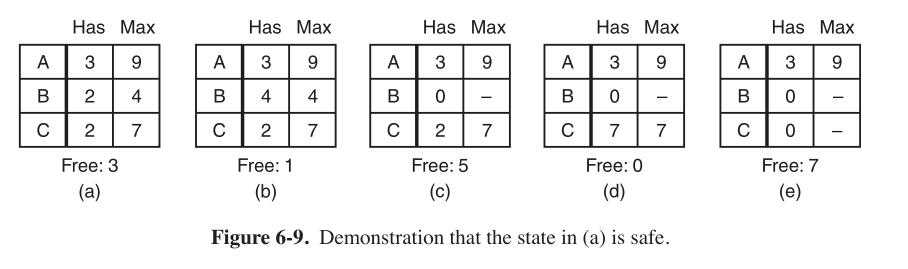
\includegraphics{safe.png}
  \end{subfigure} \\
  \begin{subfigure}[b]{0.4\linewidth}
  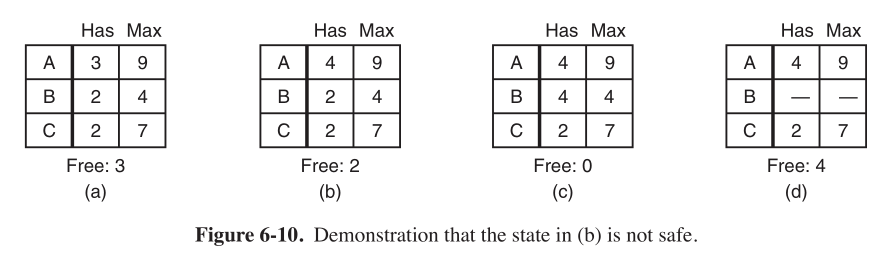
\includegraphics{unsafe.png}
  \end{subfigure}
  \caption{}
  \label{safe}
\end{figure}

\subsection{Banker's Algorithm}
其实和detection的算法几乎一样。

\subsection{Deadlock Prevention}

\begin{itemize}
\item{Mutual exclusion condition. Each resource is either currently assign-
ed to exactly one process or is available.解决这个问题就是不要把资源exclusively
分配。}
\item{Hold-and-wait condition. Processes currently holding resources that
were granted earlier can request new resources.提前说清所有的需求一次性分配。或
者在要求新的资源的时候短暂释放所有的资源。缺点是资源的分配不是最优。}
\item{No-preemption condition. Resources previously granted cannot be
forcibly taken away from a process. They must be explicitly released
by the process holding them.virtualiz resources.但不是所有都可以virtualize。}
\item{Circular wait condition. There must be a circular list of two or more
processes, each of which is waiting for a resource held by the next
member of the chain.一次只能用一个资源,但是不现实。把所有的需求进行编号,必须要
按照顺序进行request。见458页。} 
\end{itemize}

总结如\ref{deadlocksummary}.
\begin{figure}
  \centering
  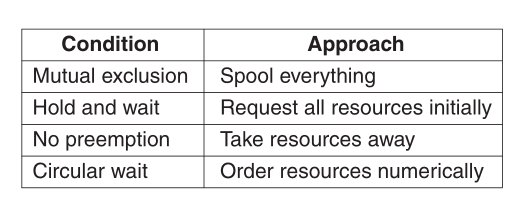
\includegraphics{deadlocksummary.png}
  \caption{}
  \label{deadlocksummary}
\end{figure}

\section{2.1 \& 2.2 Processes and Threads}
这章感觉好像没什么可考,感觉基本上都是基本的概念什么的为之后的东西做铺垫。

Thread有部分Process的特征,有自己的stack,contains the execution history. Thread
在很大程度上互相独立,但是共享一个Process environment。不同的Thread并没有不同的
Process那样独立,他们共享共同的address space,共同的global variable。不同的
Thread之间并没有互相保护。One thread could read, write or even wipe out another
thread's stack.

书上104页有一张表\ref{thread}展示了二者的区别。
\begin{figure}
  \centering
  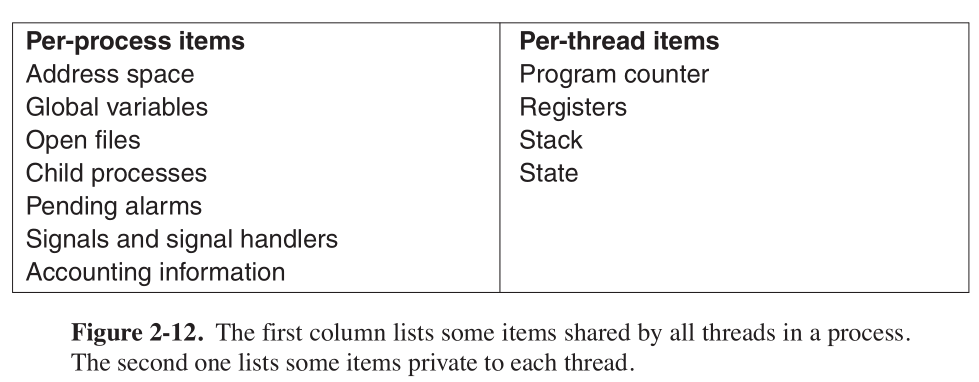
\includegraphics{thread.png}
  \caption{}
  \label{thread}
\end{figure}

假如一个thread打开了一个文件,那么另外一个thread应该是可以read这个文件的,因为
Process is the unit of resource management, not the thread.

\begin{quote}
  It is important to realize that each thread has its own stack.
\end{quote}

\subsection{Implemention of Thread}
Thread有两种implementation,一种是在user-level,由process自己实现。有几个好处。
\begin{itemize}
\item{thread switching比trapping to the kernel要快很多。}
\item{process can have customized scheduling algorithm.}
\end{itemize}

也有几个缺点,缺点主要是一些system call的问题,因为system意识不到thread的存在,所
以会选择影响整个程序。
\begin{itemize}
\item{blocking system call怎么实现是个问题。一个thread要i/o的时候假如system call
    会导致整个process block。}
\item{page fault如何handle,同样也是整个process也会被block}
\item{ In pure ULT, multithreading cannot take advantage of
    multiprocessing.\problem{这个地方我不是很理解,因为估计不同thread之间的cpu资
      源是怎么分配的可能要看具体操作系统的实现吧。}}
\end{itemize}

另外一种就是在kernel里面实现,基本上存的是process的一个子集,由于kernel创建的成
本较高,但是可以调用所有的system call 。

\subsection{State Model}
\subsubsection{Three State Model}
running, block, ready
\subsubsection{Five State Model}
new, running, block, ready, exit

\subsection{Simple Model of Multiprogramming}
\begin{figure}
  \centering
  \label{cpuutil}
  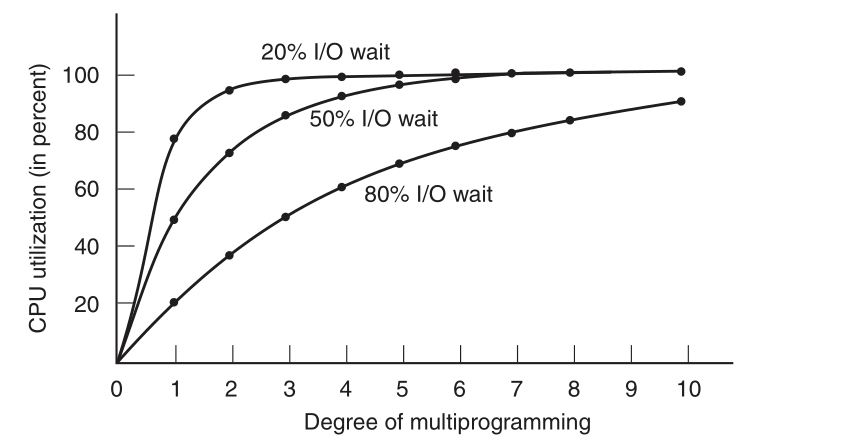
\includegraphics{cpuutil.png}
\end{figure}

\section{File Systems}
Files from a user's perspective:

File的几个属性,Naming,Structure,
\begin{description}
\item[Naming]{two-part file names} 
\item[Structure]{Byte sequence, record sequence(这个是上古punch card的遗
    留), tree(这个和record sequence差不多,只不过长度不一样,所以要换个形式组织
    罢了。)} 
\item[Type]{regular file(binary or ASCII files), directory(system files to
    maintain the structure of the file system), block special files(model disks).} 
\item[Access]{sequencial and random access(可以读取文件里的任意一个位置).} 
\item[Attributes(metadata)]{就是一些文件的属性,其实没什么可说的。} 
\end{description}

Directory感觉没什么可说的,主要是会区别hard link和symbolic link吧。

\begin{quote}
  A link of this kind, which increments the counter in the file’s
i-node (to keep track of the number of directory entries containing the
file), is sometimes called a hard link.

  A variant on the idea of linking files is the symbolic link. Instead, of having
two names point to the same internal data structure representing a file, a name can
be created that points to a tiny file naming another file.
\end{quote}

\subsection{Implementation}
感觉这个是考试的\emphasis{重点}。

\subsubsection{Layout}
文件是存在硬盘上的,一般来说硬盘都会进行分区。每个分区都有自己的结构,这个结构就
叫做layout。Sector 0总是MBR(Master Boot Record),这个是用来boot the computer. 这
个每个单独的分区。结构如图\ref{fig:disklayout}, 这里注意I-node是存在硬盘的空间里
的,并不是属于directory或者file本身的一种性质:

\begin{figure}
  \centering
  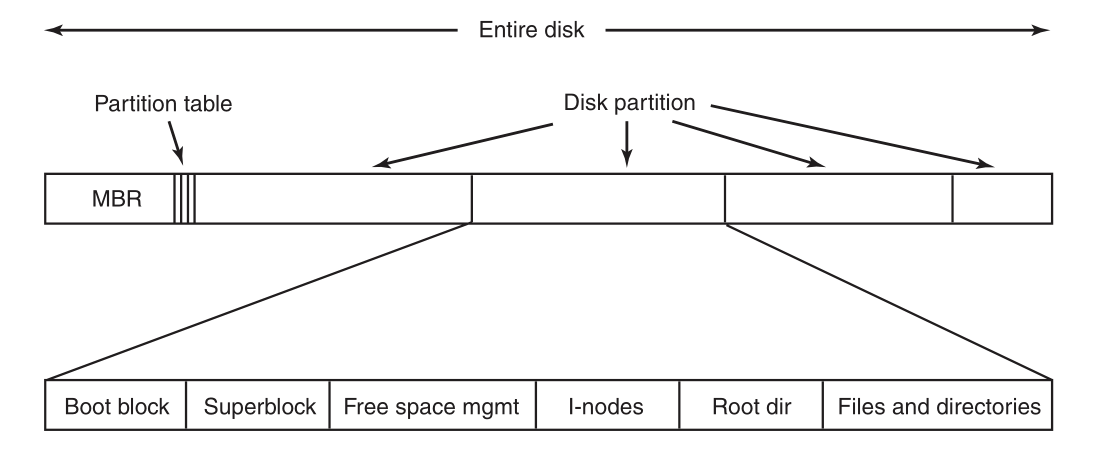
\includegraphics{disklayout.png}
  \caption{}
  \label{fig:disklayout}
\end{figure}

\subsubsection{Implementing Files: Allocation}
有两种allocation的策略,contiguous和linked-list。

contiguous:
\begin{itemize}
\item{Simple to implement.} 
\item{Read performance is excellent.} 
\item{Disk becomes fragmented.} 
\item{Need to know the final size of a file when
the file is created.} 
\end{itemize}

linked list:
\begin{itemize}
\item{No (external) fragmentation} 
\item{The directory entry needs just to store
the disk address of the first block.} 
\item{Random access is extremely slow.} 
\item{The amount of data storage is no longer
a power of two, because the pointer
takes up a few bytes.} 
\end{itemize}

由于linked list的一些缺点,演化除了所谓的FAT(File Allocation Table), 这个其实就
是把linked list里的指针单独拿出来存在一张表里然后一口气读到内存里。所以缺点是
does not scale to large disks.

\subsubsection{I-node}
\emphasis{这应该是非lab里的重中之重。}I-node是和每个file associated的,纪录了
file attribute和block disk address, 和FAT相比的优点是\emphasis{Need only be in
  memory when the corresponding file is open.}, 也就是\emphasis{file metadata.}

\subsection{Implementing Directories}
Directory其实就是mapping name to I-node的过程,以前都是比较短的file name。对于比
较长的话有两种方案\ref{longfilename},可以用hash加快寻找速度。

\begin{figure}
  \centering
  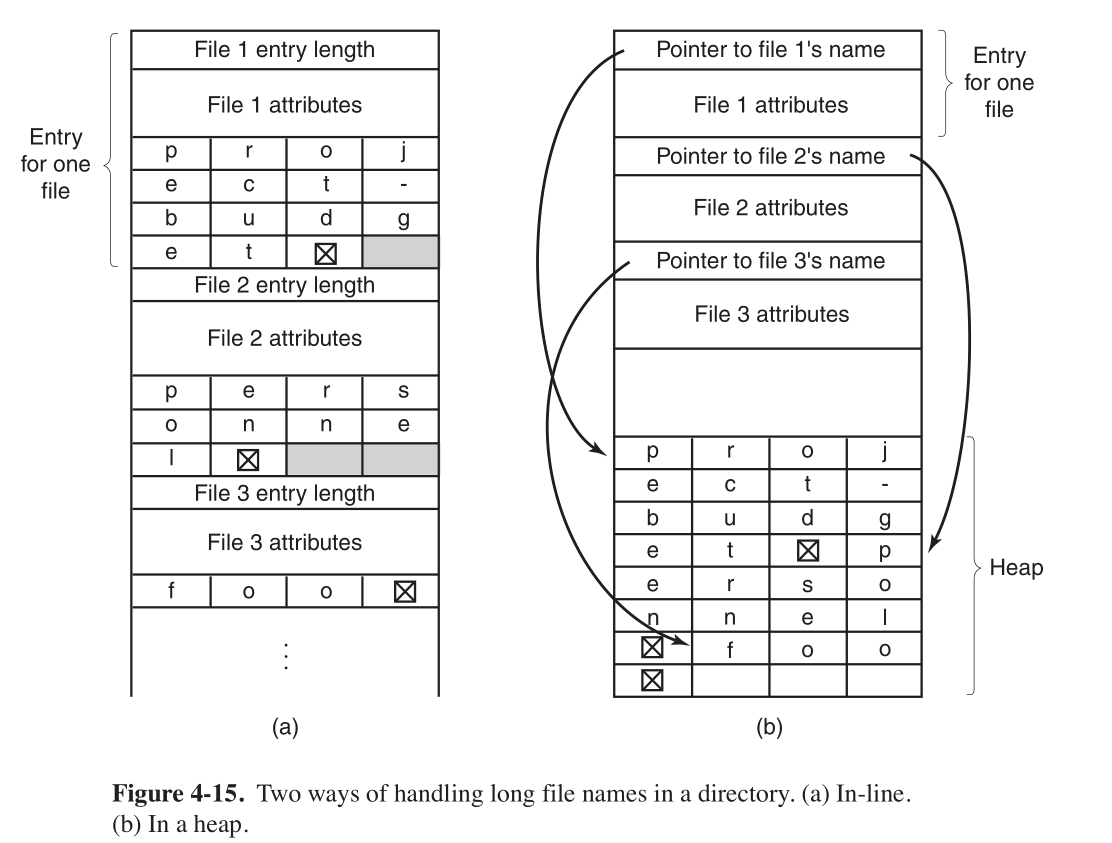
\includegraphics{longfilename.png}
  \caption{}
  \label{longfilename}
\end{figure}

\subsubsection{Shared Files}
两个用户同时使用一个文件。第一种解决方案hard link,增加了i-node的count number,
但是C假如删了这个文件之后,B面临一个invalid i-node.对i-node来说也不可能找到
directory entry(dentry)来删除它。因为没有从i-node指向direcrtory的pointer,否则太
多了存不下。

symbolic linking的是创造一个link 文件,里面存着path name指向另一个文件。

\begin{quote}
  概括来说symbolic的问题就是读起来慢,所谓的overhead,优势是可以读世界上任何一台
  机器的文件。

  The problem with symbolic links is the extra overhead required. The file con-
taining the path must be read, then the path must be parsed and followed, compo-
nent by component, until the i-node is reached. All of this activity may require a
considerable number of extra disk accesses. Furthermore, an extra i-node is needed
for each symbolic link, as is an extra disk block to store the path, although if the
path name is short, the system could store it in the i-node itself, as a kind of opti-
mization. Symbolic links have the advantage that they can be used to link to files
on machines anywhere in the world, by simply providing the network address of
the machine where the file resides in addition to its path on that machine.
\end{quote}

\begin{figure}
  \centering
  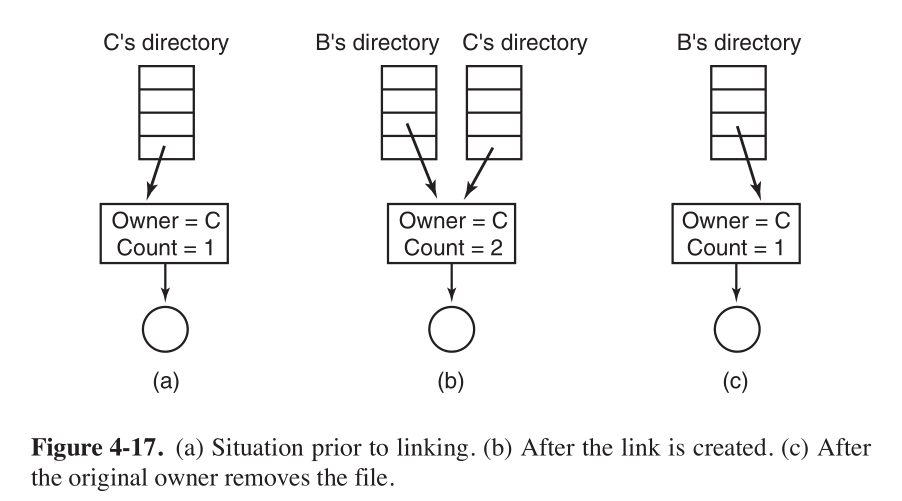
\includegraphics{staticlink.png}
  \caption{}
  \label{staticlink}
\end{figure}

\subsubsection {Log-structured and journaling}
这个初中是writing太慢了,所以吧writing攒着一起写,i-node散落在各处。

衍生出jounaling,保证文件系统的安全。

\subsection{Management and Optimization}
Block Size,越大越快,越浪费空间。越小越慢,越节约空间。

\subsubsection{Backup}
incremental dumps. physical dump. logical dump.

其他两个没什么好说的,就logical dump可以提一下。

\begin{qutoe}
  Starts at one or more specified
directories
• Recursively dumps all files and
directories found there and have
changed since some given base date.
\end{qutoe}
\nocite{*}
% \bibliography{report}{}
% \bibliographystyle{plain}
\end{document}

